\documentclass{article}

\usepackage{graphicx}
\usepackage{enumerate}

\title{Homework 3:  HTTP and HTML}

\begin{document}
\maketitle
Due Tuesday, July 30th.
Your submission for this homework should consist of three parts:
\begin{enumerate}
\item A text file or piece of paper with the \texttt{HTTP} requests from problem 1.
\item A copy of your HTML Tags sheet (you probably want to keep your original while I grade).
\item An {\bf emailed} copy of your table for problem 2 part c, in a file called \texttt{mult.html}.
\end{enumerate}

\section{HTTP (Monday)}
Construct an HTTP request which fetches each of the following things.  You should use the \texttt{http\_request.py} script also posted on the website.  I will demo using it in class.  All of these should give you an HTTP response code of 200.  If you're getting 301 (redirects) or 404 (not found) you don't yet have the right answer.
\begin{enumerate}[a]
\item The class website (you shouldn't have to modify the script to do this).
\item Last week's homework assignment from the class webpage.  You should be able to see a lot of unreadable stuff in the response which is pdf data not meant to be read by humans.
\item Try requesting the class website, but removing the host header.  What does your request look like, and what do you get?
\item The ESP homepage (esp.mit.edu/index.html)
\item Try using the \texttt{HEAD} HTTP request method.  To do this, just replace \texttt{GET} with \texttt{HEAD} in the request.  Try it on a few websites.  What does it do?
\item Challenge:  Get the ESP homepage with you logged in using the python script.  You should use the ``cookie'' header.  When you turn this one in, don't write the whole cookie down, just \texttt{cookie} where you put the actual cookie.  Hint:  Look at the requests the ESP website is sending using chrome developer tools or similar.  You can tell that you succeeded when the response includes your username.
\end{enumerate}

\section{HTML (Wednesday)}

\begin{enumerate}[a]
\item Figure out what all of the tags on the HTML tag sheet do.
\item Find five more useful-looking tags and add them to the tag sheet.
\item Make an HTML document with a multiplication table up to fives.  I used the tags \texttt{<body>}, \texttt{<table>}, \texttt{<th>}, \texttt{<tr>}, and \texttt{<td>}, and no others.  It should look like this:

\end{enumerate}
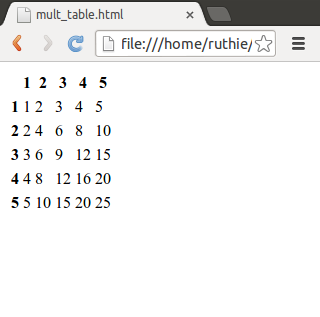
\includegraphics{mult_table_output.png}

\vspace{-3 cm}
\section{Preparation for Website Project}
Go to nearlyfreespeech.net and read or skim the following pages:
\begin{enumerate} 
\item Terms of service (\texttt{https://www.nearlyfreespeech.net/about/terms})
\item Pricing summary (\texttt{https://www.nearlyfreespeech.net/services/pricing})
\item The first FAQ question (\texttt{https://www.nearlyfreespeech.net/about/faq}), and as much else of their (very long) FAQ as you want.  Much of it is interesting.
\item (Optional) find another web hosting service and compare terms and conditions/pricing policies.
\end{enumerate}

It's important to know what the terms and price is when you use any service.  That's what ``doing your homework'' means in real life.  You don't need to hand in anything for this part, but please do it anyway.
\end{document}
